%                                                                 aa.dem
% AA vers. 9.1, LaTeX class for Astronomy & Astrophysics
% demonstration file
%                                                       (c) EDP Sciences
%-----------------------------------------------------------------------
%
% \documentclass[referee]{aa} % for a referee version
%\documentclass[onecolumn]{aa} % for a paper on 1 column  
%\documentclass[longauth]{aa} % for the long lists of affiliations 
%\documentclass[letter]{aa} % for the letters 
%\documentclass[bibyear]{aa} % if the references are not structured 
%                              according to the author-year natbib style

%

\documentclass{aa}  

%
\usepackage{graphicx}
\usepackage{amsmath,amsfonts,amssymb}
\usepackage{natbib}


%%%%%%%%%%%%%%%%%%%%%%%%%%%%%%%%%%%%%%%%
\usepackage{txfonts}
\usepackage{xcolor}

\usepackage{blindtext}
%%%%%%%%%%%%%%%%%%%%%%%%%%%%%%%%%%%%%%%%
% \usepackage[options]{hyperref}
% To add links in your PDF file, use the package "hyperref"
% with options according to your LaTeX or PDFLaTeX drivers.
\usepackage{float}
%\usepackage{stfloats}
\usepackage{dblfloatfix}
\usepackage{afterpage}
\usepackage{ifthen}
\usepackage[morefloats=12]{morefloats}

\usepackage{placeins}
\usepackage{multicol}
%\usepackage[breaklinks,colorlinks,citecolor=blue]{hyperref}
\bibpunct{(}{)}{;}{a}{}{,}
\usepackage[switch]{lineno}
\definecolor{linkcolor}{rgb}{0.6,0,0}
\definecolor{citecolor}{rgb}{0,0,0.75}
\definecolor{urlcolor}{rgb}{0.12,0.46,0.7}
\usepackage[breaklinks, colorlinks, urlcolor=urlcolor,
    linkcolor=linkcolor,citecolor=citecolor,pdfencoding=auto]{hyperref}
\hypersetup{linktocpage}
\usepackage{bold-extra}

%Planck style file, to be used with A&A style to produce Planck papers for publication.
%
% version 28 September 2010 --- useful macros --- CRL
% version 17 October 2010   --- first cut at important instrument values, from Daniele Mennella and
%                               Francois Bouchet, 13 October 2010 --- CRL
% version 18 October 2010   --- LFI FWHM changed to one value per feed, rather than M & S separately
%                               LFI FWHM uncertainties added for individual feeds.  Corrections made
%                               to LFI values. --- Andrea Zacchei
% version 24 October 2010   --- added to and corrected definitions.  No changes made to instrument
%                               quantities. --- CRL 
% version 31 October 2010   --- added definition of \muKHz. --- CRL
%
% version 15 November 2010  --- fixed conflict with aa.cls in definition of \endtable
%                               by naming the command below "\endPlancktable".  See section
%                               13.16 of the Style Guide.
%
% version 06 December 2010  --- Set up names with and without units.
%                               Add \allearlypapers command to ensure that all early papers are
%                               included in the reference list.
%                               Define macro for the name of the 4He JT cooler.
%
% version 07 December 2010  --- removed extraneous "planck2011-1.2" entry in \allearlypapers
%
% version 12 December 2010  --- added \endPlancktablewide command to set tablenotes to the full
%                               page width in the \begin{table*}...\end{table*} environment when
%                               the ``twocolumn'' option is specified in the \documentclass command.
%                               (It would be more elegant to extract the appropriate width from the
%                               aa.cls system at the time of execution, but that is buried more
%                               deeply in the system than I investigated.)
%
% version 05 January 2011   --- added unit \MJysr.  HFI performance values updated per FRB email
%                               01/05/2011 02:38-0800, and Brendan Crill email 01/05/2011 18:08 -0800.
%
% version 06 January 2011   --- changed \scriptscriptstyle primes to \scriptstyle, to better match the
%                               tx fonts used by A&A.
%
% version 07 January 2011   --- modified \allearlypapers to correspond with final early paper list.  
%                               Fixed 545 GHz center frequency.
%
% version 07 January 2011b  --- changed LFI white-noise sensitivity numbers to correct problem with units
%
% version 05 July 2011      --- added \Msol and \Lsol to get the symbols for solar mass and luminosity.
%                               Deleted previous definitions of \solar and \sol, which were equivalent
%                               to the new \Msol.
%
% version 16 August 2011    --- changed comments on \endPlancktable and \endPlancktablewide for clarity
%
% version 11 September 2011 --- changed definition of \tablenote to make footnote labels italic, as per A\&A
%
% version 26 April 2011     --- changed definition of \Planck to agree with what is said in the Style Guide (!)
%
% version 04 Dec 2013       --- included 2013 results references
%
% version 17 Jan 2014       --- included fix to bibtex file v4.3, i.e. \providecommand{\sorthelp}[1]{}
%
% version 26 Jul 2014       --- fixed incompatibility problem with aa.cls v8.0 and v8.2.  v8.2 should now be used
%                               for all Planck papers.
%                           --- fixed problem in definition of "\all2013resultspapers" that introduced a blanck
%                               into the reference to p06b.
%                           --- removed all the parameter definition stuff at the end.  We weren't using it, and
%                               it took up a lot of space.
%
% version 28 Jan 2015       --- added "\alltwentyfiftennresultspapers" and corrected "\all2013resultspapers" to
%                               "\all20thirteenresultspapers",
%
% Usage:  after the \documentclass[traditabstract]{aa} command in the La\TeX\ input file,
%         add this command:      \input Planck.tex


\def\setsymbol#1#2{\expandafter\def\csname #1\endcsname{#2}}
\def\getsymbol#1{\csname #1\endcsname}

%-----------------------------------------------------------------------
% Planck
%-----------------------------------------------------------------------
\def\Planck{\textit{Planck}}

%-----------------------------------------------------------------------
% The Planck Helium-4 JT cooler
%-----------------------------------------------------------------------
\def\HeJT{$^4$He-JT}

%-----------------------------------------------------------------------
% To include all Planck Early Results papers in the reference lists
%-----------------------------------------------------------------------
\def\allearlypapers{\nocite{planck2011-1.1, planck2011-1.3, planck2011-1.4, planck2011-1.5, planck2011-1.6, planck2011-1.7, planck2011-1.10, planck2011-1.10sup, planck2011-5.1a, planck2011-5.1b, planck2011-5.2a, planck2011-5.2b, planck2011-5.2c, planck2011-6.1, planck2011-6.2, planck2011-6.3a, planck2011-6.4a, planck2011-6.4b, planck2011-6.6, planck2011-7.0, planck2011-7.2, planck2011-7.3, planck2011-7.7a, planck2011-7.7b, planck2011-7.12, planck2011-7.13}}

%-----------------------------------------------------------------------
% To include all Planck 2013 Results papers in the reference lists
%-----------------------------------------------------------------------
\def\alltwentythirteenresultspapers{\nocite{planck2013-p01, planck2013-p02, planck2013-p02a, planck2013-p02d, planck2013-p02b, planck2013-p03, planck2013-p03c, planck2013-p03f, planck2013-p03d, planck2013-p03e, planck2013-p01a, planck2013-p06, planck2013-p03a, planck2013-pip88, planck2013-p08, planck2013-p11, planck2013-p12, planck2013-p13, planck2013-p14, planck2013-p15, planck2013-p05b, planck2013-p17, planck2013-p09, planck2013-p09a, planck2013-p20, planck2013-p19, planck2013-pipaberration, planck2013-p05, planck2013-p05a, planck2013-pip56, planck2013-p06b, planck2013-p01a}}

%-----------------------------------------------------------------------
% To include all Planck 2015 Results papers in the reference lists
%-----------------------------------------------------------------------
\def\alltwentyfifteenresultspapers{\nocite{planck2014-a01, planck2014-a03, planck2014-a04, planck2014-a05, planck2014-a06, planck2014-a07, planck2014-a08, planck2014-a09, planck2014-a11, planck2014-a12, planck2014-a13, planck2014-a14, planck2014-a15, planck2014-a16, planck2014-a17, planck2014-a18, planck2014-a19, planck2014-a20, planck2014-a22, planck2014-a24, planck2014-a26, planck2014-a28, planck2014-a29, planck2014-a30, planck2014-a31, planck2014-a35, planck2014-a36, planck2014-a37, planck2014-ES}}

%-----------------------------------------------------------------------
% Tables
%-----------------------------------------------------------------------
\newbox\tablebox    \newdimen\tablewidth
\def\leaderfil{\leaders\hbox to 5pt{\hss.\hss}\hfil}
%
% use the following definition of \endPlancktable for ApJ style notes to tables, set to the 
%         width of the table
% \def\endPlancktable{\tablewidth=\wd\tablebox 
%
% use the following definitions of \endPlancktable and \endPlancktablewide for A&A style notes 
% set to one-column  or full-page width, respectively
\def\endPlancktable{\tablewidth=\columnwidth 
    $$\hss\copy\tablebox\hss$$
    \vskip-\lastskip\vskip -2pt}
\def\endPlancktablewide{\tablewidth=\textwidth 
    $$\hss\copy\tablebox\hss$$
    \vskip-\lastskip\vskip -2pt}
\def\tablenote#1 #2\par{\begingroup \parindent=0.8em
    \abovedisplayshortskip=0pt\belowdisplayshortskip=0pt
    \noindent
    $$\hss\vbox{\hsize\tablewidth \hangindent=\parindent \hangafter=1 \noindent
    \hbox to \parindent{$^#1$\hss}\strut#2\strut\par}\hss$$
    \endgroup}
\def\doubleline{\vskip 3pt\hrule \vskip 1.5pt \hrule \vskip 5pt}

%-----------------------------------------------------------------------
% useful macros
%-----------------------------------------------------------------------
%
\def\L2{\ifmmode L_2\else $L_2$\fi}
%
\def\dtt{\Delta T/T}
\def\DeltaT{\ifmmode \Delta T\else $\Delta T$\fi}
\def\deltat{\ifmmode \Delta t\else $\Delta t$\fi}
\def\fknee{\ifmmode f_{\rm knee}\else $f_{\rm knee}$\fi}
\def\Fmax{\ifmmode F_{\rm max}\else $F_{\rm max}$\fi}
%
\def\solar{\ifmmode{\rm M}_{\mathord\odot}\else${\rm M}_{\mathord\odot}$\fi}
\def\Msolar{\ifmmode{\rm M}_{\mathord\odot}\else${\rm M}_{\mathord\odot}$\fi}
\def\Lsolar{\ifmmode{\rm L}_{\mathord\odot}\else${\rm L}_{\mathord\odot}$\fi}
%
\def\inv{\ifmmode^{-1}\else$^{-1}$\fi}
\def\mo{\ifmmode^{-1}\else$^{-1}$\fi}
\def\sup#1{\ifmmode ^{\rm #1}\else $^{\rm #1}$\fi}
\def\expo#1{\ifmmode \times 10^{#1}\else $\times 10^{#1}$\fi}
%
\def\,{\thinspace}
\def\lsim{\mathrel{\raise .4ex\hbox{\rlap{$<$}\lower 1.2ex\hbox{$\sim$}}}}
\def\gsim{\mathrel{\raise .4ex\hbox{\rlap{$>$}\lower 1.2ex\hbox{$\sim$}}}}
\let\lea=\lsim
\let\gea=\gsim
\def\simprop{\mathrel{\raise .4ex\hbox{\rlap{$\propto$}\lower 1.2ex\hbox{$\sim$}}}}
%
\def\deg{\ifmmode^\circ\else$^\circ$\fi}
\def\pdeg{\ifmmode $\setbox0=\hbox{$^{\circ}$}\rlap{\hskip.11\wd0 .}$^{\circ}
          \else \setbox0=\hbox{$^{\circ}$}\rlap{\hskip.11\wd0 .}$^{\circ}$\fi}
\def\arcs{\ifmmode {^{\scriptstyle\prime\prime}}
          \else $^{\scriptstyle\prime\prime}$\fi}
\def\arcm{\ifmmode {^{\scriptstyle\prime}}
          \else $^{\scriptstyle\prime}$\fi}
\newdimen\sa  \newdimen\sb
\def\parcs{\sa=.07em \sb=.03em
     \ifmmode \hbox{\rlap{.}}^{\scriptstyle\prime\kern -\sb\prime}\hbox{\kern -\sa}
     \else \rlap{.}$^{\scriptstyle\prime\kern -\sb\prime}$\kern -\sa\fi}
\def\parcm{\sa=.08em \sb=.03em
     \ifmmode \hbox{\rlap{.}\kern\sa}^{\scriptstyle\prime}\hbox{\kern-\sb}
     \else \rlap{.}\kern\sa$^{\scriptstyle\prime}$\kern-\sb\fi}
%
\def\ra[#1 #2 #3.#4]{#1\sup{h}#2\sup{m}#3\sup{s}\llap.#4}
\def\dec[#1 #2 #3.#4]{#1\deg#2\arcm#3\arcs\llap.#4}
\def\deco[#1 #2 #3]{#1\deg#2\arcm#3\arcs}
\def\rra[#1 #2]{#1\sup{h}#2\sup{m}}
%
\def\page{\vfill\eject}
\def\dots{\relax\ifmmode \ldots\else $\ldots$\fi}
%
%-----------------------------------------------------------------------
% units
%-----------------------------------------------------------------------
%
\def\WHzsr{\ifmmode $W\,Hz\mo\,sr\mo$\else W\,Hz\mo\,sr\mo\fi}
\def\mHz{\ifmmode $\,mHz$\else \,mHz\fi}
\def\GHz{\ifmmode $\,GHz$\else \,GHz\fi}
\def\mKs{\ifmmode $\,mK\,s$^{1/2}\else \,mK\,s$^{1/2}$\fi}
\def\muKs{\ifmmode \,\mu$K\,s$^{1/2}\else \,$\mu$K\,s$^{1/2}$\fi}
\def\muKRJs{\ifmmode \,\mu$K$_{\rm RJ}$\,s$^{1/2}\else \,$\mu$K$_{\rm RJ}$\,s$^{1/2}$\fi}
\def\muKHz{\ifmmode \,\mu$K\,Hz$^{-1/2}\else \,$\mu$K\,Hz$^{-1/2}$\fi}
\def\MJysr{\ifmmode \,$MJy\,sr\mo$\else \,MJy\,sr\mo\fi}
\def\MJysrmK{\ifmmode \,$MJy\,sr\mo$\,mK$_{\rm CMB}\mo\else \,MJy\,sr\mo\,mK$_{\rm CMB}\mo$\fi}
\def\microns{\ifmmode \,\mu$m$\else \,$\mu$m\fi}
\def\micron{\microns}
\def\muK{\ifmmode \,\mu$K$\else \,$\mu$\hbox{K}\fi}
\def\microK{\ifmmode \,\mu$K$\else \,$\mu$\hbox{K}\fi}
\def\muW{\ifmmode \,\mu$W$\else \,$\mu$\hbox{W}\fi}
\def\kms{\ifmmode $\,km\,s$^{-1}\else \,km\,s$^{-1}$\fi}
\def\kmsMpc{\ifmmode $\,\kms\,Mpc\mo$\else \,\kms\,Mpc\mo\fi}
%
%
%----------------------------------------------------------------------
% set up machinery to list Planck papers in roman numeral order.
%----------------------------------------------------------------------

\providecommand{\sorthelp}[1]{}


% Custom definitions
\newcommand{\mathsc}[1]{{\normalfont\textsc{#1}}}
\def\Cosmoglobe{\textsc{Cosmoglobe}}
\def\Planck{\textit{Planck}}
\def\WMAP{\textit{WMAP}}


\begin{document} 


   \title{\bfseries{\Cosmoglobe\ DR2. IV. Modelling starlight emission\\ in DIRBE with GAIA and WISE}}

   \author{Placeholder}

   \institute{Institute of Theoretical Astrophysics, University of Oslo, Blindern, Oslo, Norway}
  
   % Shortened title, author list for top of page 
   \titlerunning{Starlight emission in DIRBE}
   \authorrunning{Placeholder}

   \date{\today} 
   
   \abstract{We present a model of starlight emission in the Diffuse Infrared Background Explorer (DIRBE) data between 1.25 and 25$\,\mu$m based on GAIA and WISE measurements. For each star brighter than magnitude 8 in the WISE 3.4$\,\mu$m band, we extract estimates of the effective temperature, $T_{\mathrm{eff}}$, the gravitational acceleration, $\log g$, and the metallicity, $[M/H]$, from the GAIA DR2 database, and use those to identify a best-fit spectral energy density (SED) from the PHOENIX starlight database. This SED is convolved with the appropriate DIRBE bandpasses and beam response function, and only a single overall flux density is fitted per star. We find that the number of stars with a statistically significant flux density detected at Galactic latitudes $|b|>20^{\circ}$ at more than than $5\,\sigma$ is 313\,061 stars, for an average of 0.4~stars per DIRBE beam area. Furthermore, based on this model we find that total star emission accounts for 98\,\% of the observed flux density at 1.25\,$\mu$m; 83\,\% at 4.9$\,\mu$m; and 3\,\% at 25\,$\mu$m. As shown in companion papers, this new model is sufficiently accurate to allow for precise characterization of both extragalactic background (cosmic infrared and optical background; CIB and COB) fluctuations and Galactic (free-free and polycyclic aromatic hydrocarbon (PAH) dust) emission in the four highest DIRBE frequencies.      }

   \keywords{ISM: general - Zodiacal dust, Interplanetary medium - Cosmology: observations, diffuse radiation - Galaxy: general}

   \maketitle

\setcounter{tocdepth}{2}
\tableofcontents
   
% INTRODUCTION
%-------------------------------------------------------------------
\section{Introduction}
%\the\textwidth \the\columnwidth

Modelling the microwave sky in the COBE-Diffuse Infrared Background Explorer (DIRBE) data  \citep{DIRBE} from 1 to 100000 GHz requires a  understanding of all the various components that make it up. At the highest frequencies, the largest power contribution comes from stars in our galaxy, as can be seen in Fig. \ref{fig:sed}. The smallest wavelength/highest frequency bands 1-4 are dominated by star emissions, making accurate star modelling essential for using these data in combination with others in a comprehensive Bayesian model of the large-scale infrared sky. Additionally, stars are subdominant contributors in DIRBE bands 5 and 6, which if not handled correctly could heavily skew derived constraints on the zodiacal light and other components.

Many full-sky datasets exist which measure the emissions from stars in our galaxy. Staring with IRAS in 1983 \citep{iras}, there have been several ground and space missions to map the infrared sky and put constraints on star star formation and evolution, the Cosmic Infrared Background (CIB) and Active Galactic Nuclei (AGN), including the Infrared Space Observatory (ISO) \citep{iso}, Spitzer \citep{spitzer}, the 2-Micron All-Sky Survey (2MASS) \citep{2mass}, and the current-generation James Webb Space Telescope \citep{jwst}. For the purposes of compatibility with the DIRBE data, however, the most useful external datasets are the Wide-Field Infrared Survey Explorer (WISE) \citep{wise}, and GAIA, which produced high precision star observations at optical wavelengths \citep{gaia}. 

\begin{figure*}
  \centering
  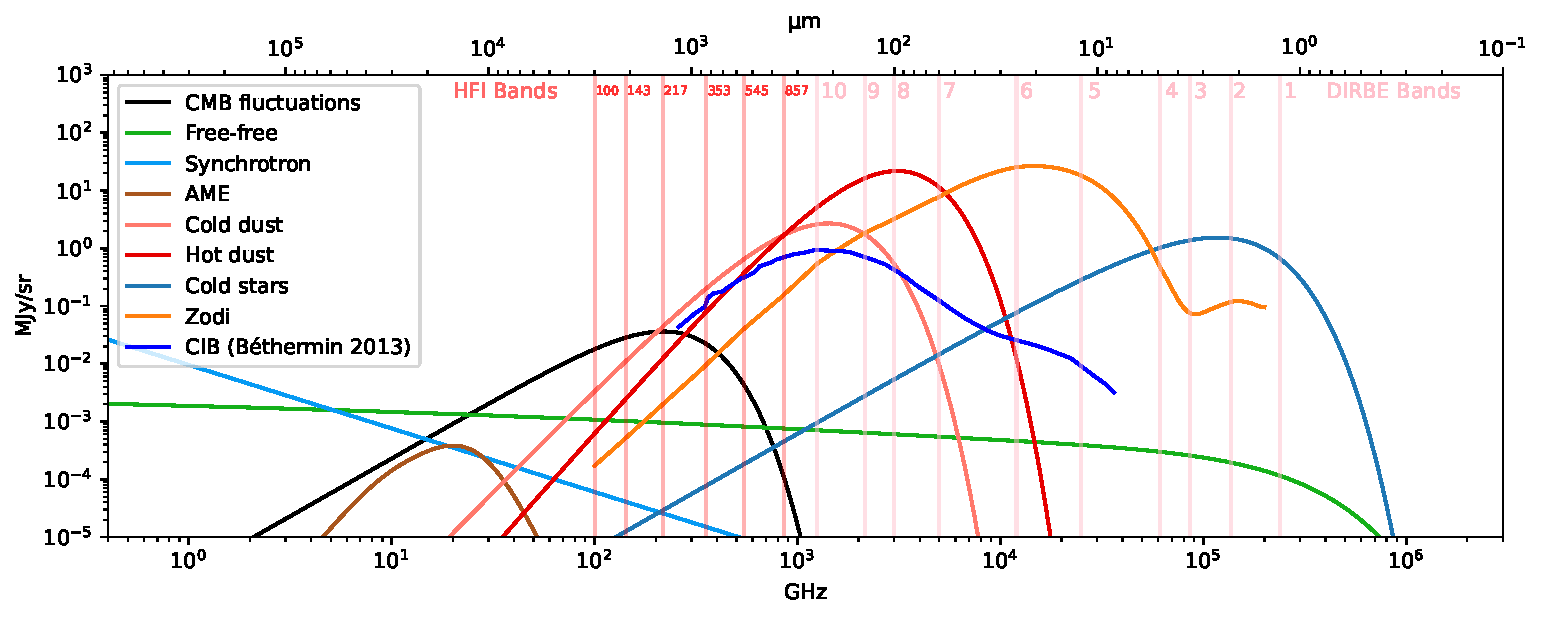
\includegraphics[width=\textwidth]{figs/sed/all_fgs.pdf}
  \caption{Components of the infrared temperature sky from 0.1$\mu$m to 1m wavelengths. The approximate contribution from stars is shown in blue, and the DIRBE and HFI band nominal frequencies are indicated by the vertical lines.}
  \label{fig:sed}
\end{figure*}

In this paper, part of the larger Cosmoglobe DR2 results paper suite, we discuss the modelling of stars as part of our larger full sky astrophysical model. Section \ref{sec:models} discusses star modelling in a larger Bayesian context. Section \ref{sec:impact} then shows the impact of stars on the DIRBE data. Section \ref{sec:data} discusses the data selection and cleaning used in our analysis, and then Section \ref{sec:results} shows the astrophysical results of the work by presenting a unified star model and its associated errors. Finally, we conclude in Section \ref{sec:conclusions}, and offer some avenues for future research.

\section{Star modelling in a Bayesian context}
\label{sec:models}

The full Bayesian data mode is shown in \cite{CG02_01}, and includes the star component $s_{stars}(p, \lambda_j)$, the star emissions as a function of pixel $p$ and frequency $\lambda_j$ for a band $j$. Equation \ref{eq:datamodel} shows the data model for the star component that we describe in this paper

\begin{equation}
s_{stars}(p, \lambda_j) = \sum_i a_i B_i(p, \lambda_j) E_i(\lambda_j).
\label{eq:datamodel}
\end{equation}

Here, we sum over each star $i$, where $a_i$ is a single overall amplitude parameter fit per star and $B_i(p, \lambda)$ is the instrument beam for a detector at frequency $\lambda$ in a pixel $p$ for a given star $i$. $E_i(\lambda)$ is the normalized emission for a given frequency $\lambda$. The emission $E_i$ is drawn directly from the GAIA data and the PHOENIX starlight database (see Sec. \ref{sec:catalogue}), and the beam $B$ is fixed for each detector, so we fit only the overall amplitude $a_i$ for each star in this model. This greatly reduces the degeneracies between the stars and other astrophysical components such as dust, and was found to work better than fitting a full SED per star (Sec. \ref{sec:impact}). We include a star component in DIRBE bands 01-06, as at longer wavelengths the contribution from star emission was greatly subdominant to zodiacal light and dust, and including that data degraded the quality of the amplitude fits. 

To sample the star amplitudes $a_i$ we attempt to minimize the residual in each band for each source $i$

\begin{equation}
\label{eq:minimize}
X_ia_i - Y_i = 0.
\end{equation}

The solution is just the mapmaking equation, where

\begin{equation}
X_i = S^T N^{-1} S = \sum_{j,p}\frac{E_{ij}^2 B^2_{ij}(p)}{\sigma_j^2(p)} 
\end{equation}

and

\begin{equation}
Y_i = S^TN^{-1}d = \sum_{j,p} \frac{E_{ij}B_{ij}(p) d_j(p)}{\sigma_j^2(p)}.
\end{equation}

Here, $\sigma_j^2(p)$ is the noise in pixel $p$ in band $j$, and $d_j(p)$ is the data map in band $j$ at pixel $p$. To reduce degeneracies, we fit the point sources on a data map with all other astrophysical components already removed, so $d_j(p)$ contains only noise and the point source $i$. The solution to \ref{eq:minimize} is simply $a_i = \frac{Y_i}{X_i}$, which gives a single overall amplitude for each star $i$. To sample the amplitudes, we also include a fluctuation term, such that our final sample for the amplitudes is given by

\begin{equation}
a_i = \frac{Y_i}{X_i} + \frac{1}{\sqrt{X_i}} N_i(0,1),
\end{equation}

where $N_i(0,1)$ is a sample drawn from a unit Gaussian with 0 mean.


\section{Impact of starlight on DIRBE observations}
\label{sec:impact}

The DIRBE data contain 

%\begin{figure}
%  \centering
%  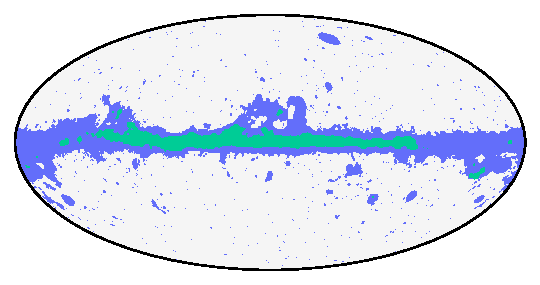
\includegraphics[width=\columnwidth]{figs/mask_proc_calib.pdf}
%  \caption{Processing masks use in the analysis.}
%  \label{fig:masks}
%\end{figure}

Diffuse stars vs. point sources? 



\clearpage
\section{Data selection and cleaning}
\label{sec:data}

The results presented in Section \ref{sec:results} are a part of the Cosmoglobe DR2 release. Here we will discuss only the data selection specific to star modelling, for a full overview of Cosmoglobe DR2, please refer to  \cite{CG02_01}.

\subsection{Catalogue Creation}
\label{sec:catalogue}

Star positions are drawn from a catalogue 

\subsection{Data Cleaning}



\clearpage
\section{Astrophysical results}
\label{sec:results}

In Figure \ref{fig:stars} we show the mean star component maps for the full pipeline run in all six DIRBE bands where stars are subtracted. 

\begin{figure*}
  \centering
%  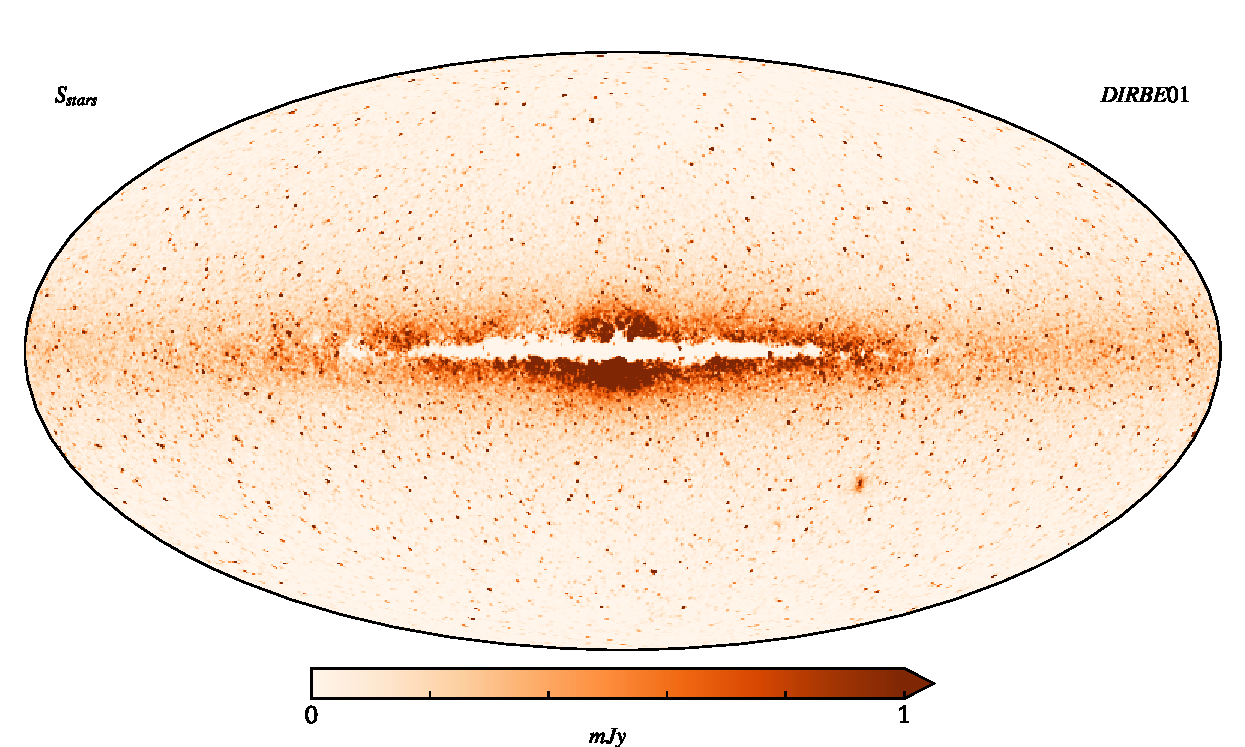
\includegraphics[width=0.49\columnwidth]{figs/stars_mean_01.pdf}
%  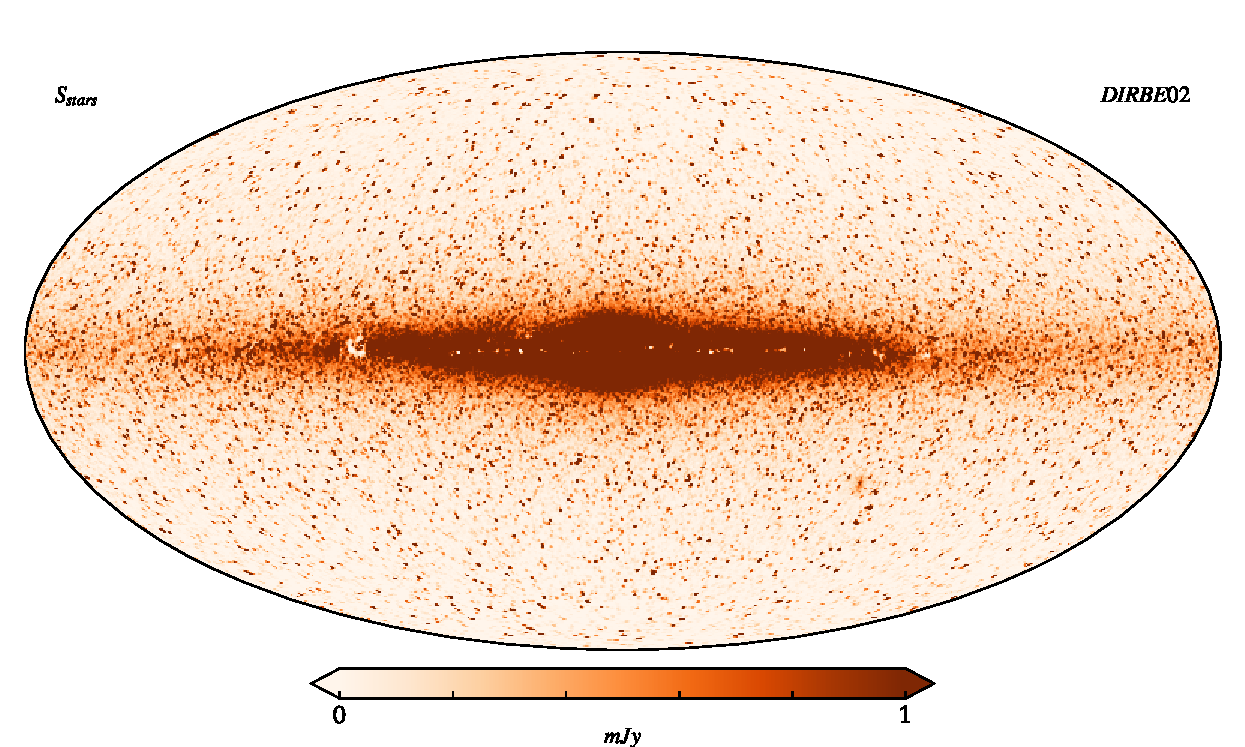
\includegraphics[width=0.49\columnwidth]{figs/stars_mean_02.pdf} \\
%  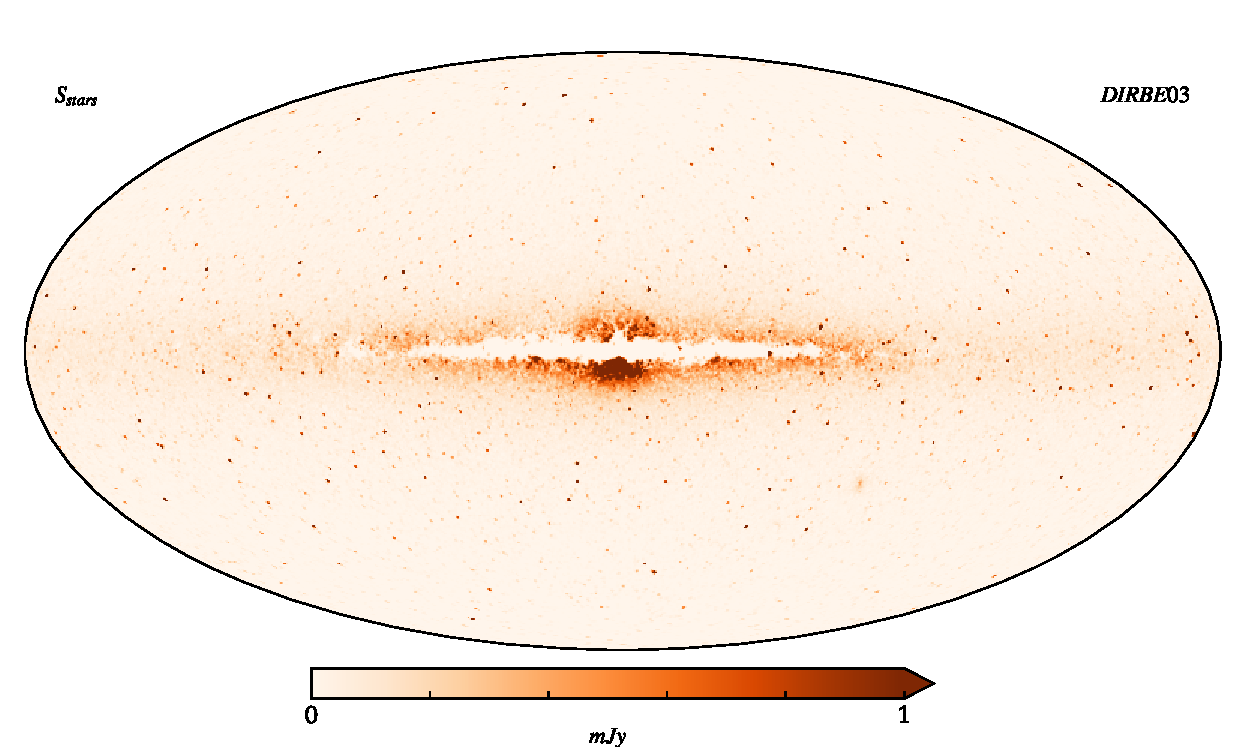
\includegraphics[width=0.49\columnwidth]{figs/stars_mean_03.pdf}
%  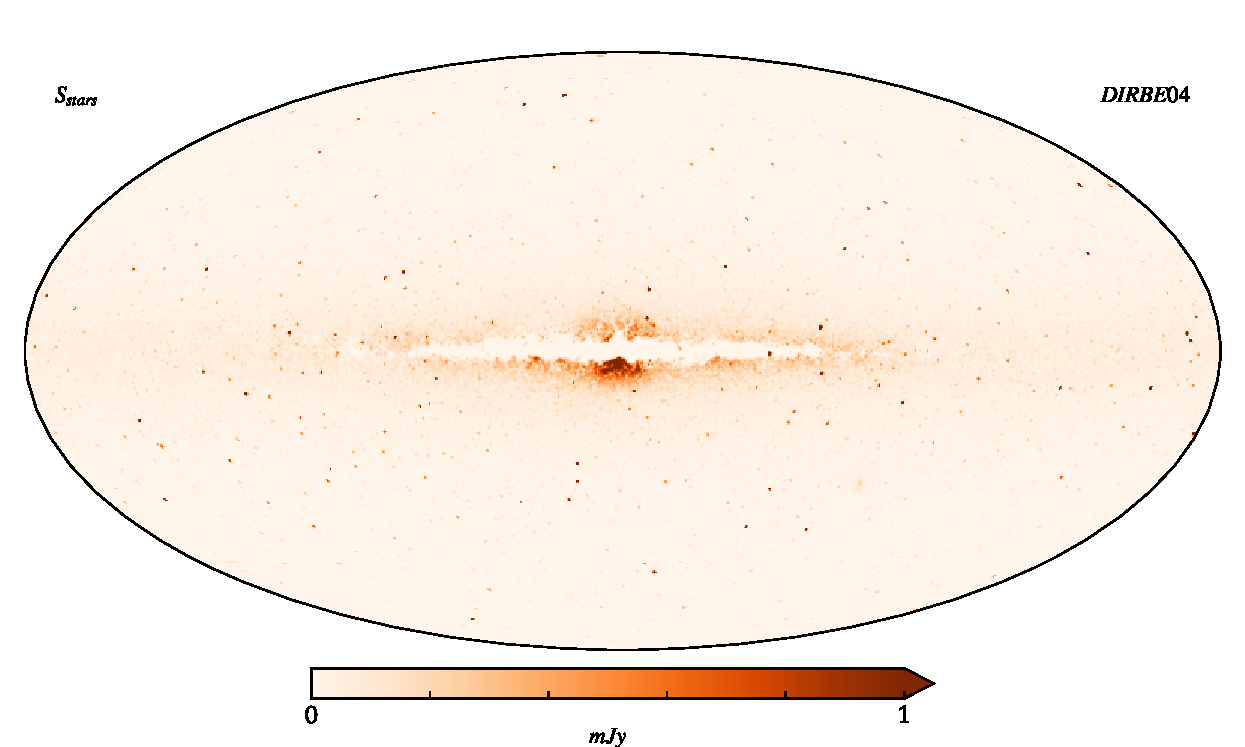
\includegraphics[width=0.49\columnwidth]{figs/stars_mean_04.pdf} \\
%  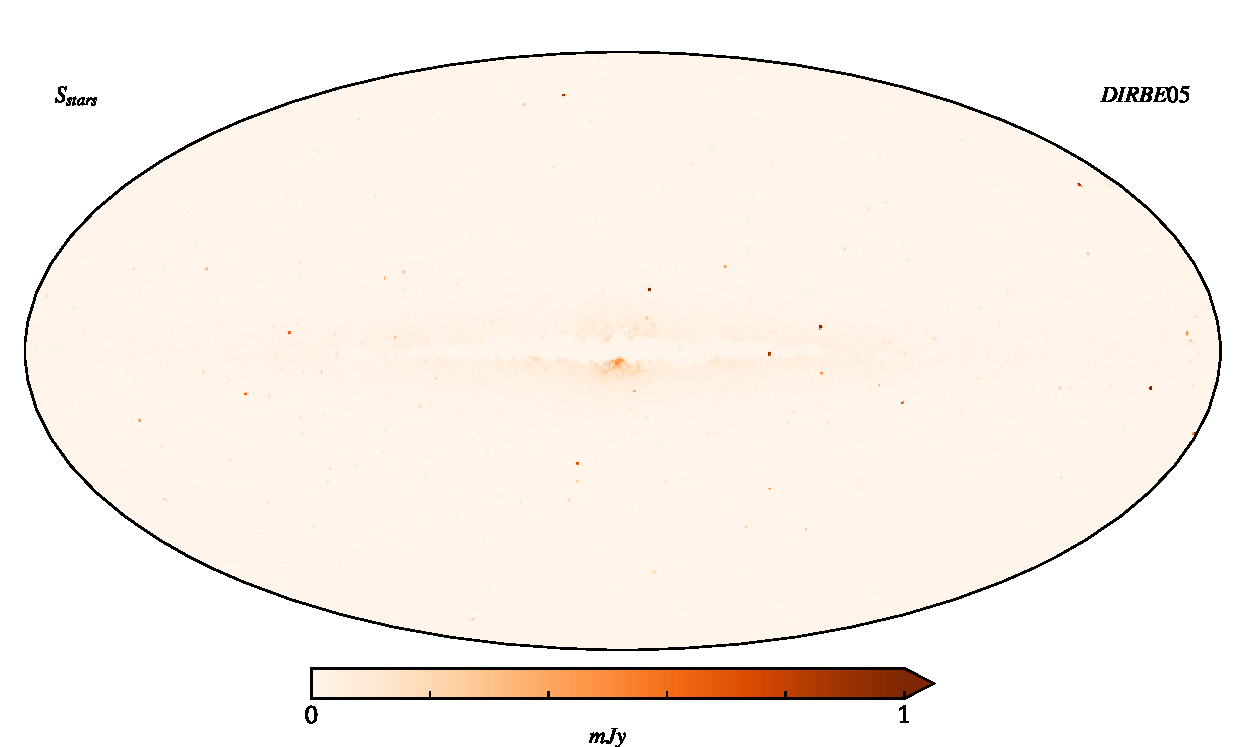
\includegraphics[width=0.49\columnwidth]{figs/stars_mean_05.pdf}
%  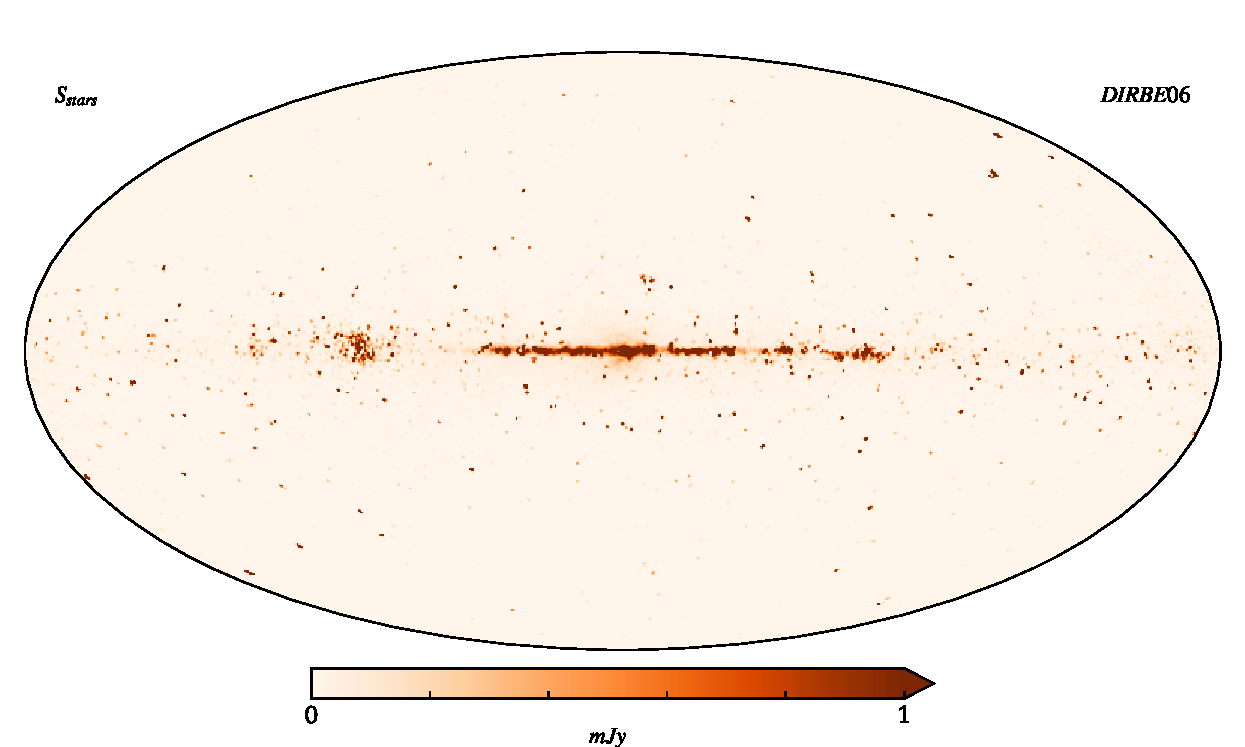
\includegraphics[width=0.49\columnwidth]{figs/stars_mean_06.pdf} \\
  \caption{Mean star maps from the Cosmoglobe DR2 release for the first 6 DIRBE bands. }
  \label{fig:stars}
\end{figure*}

In Figure \ref{fig:std} we show the standard deviations of the same data, which correspond to the errors on our star fits. 

\begin{figure*}
  \centering
%  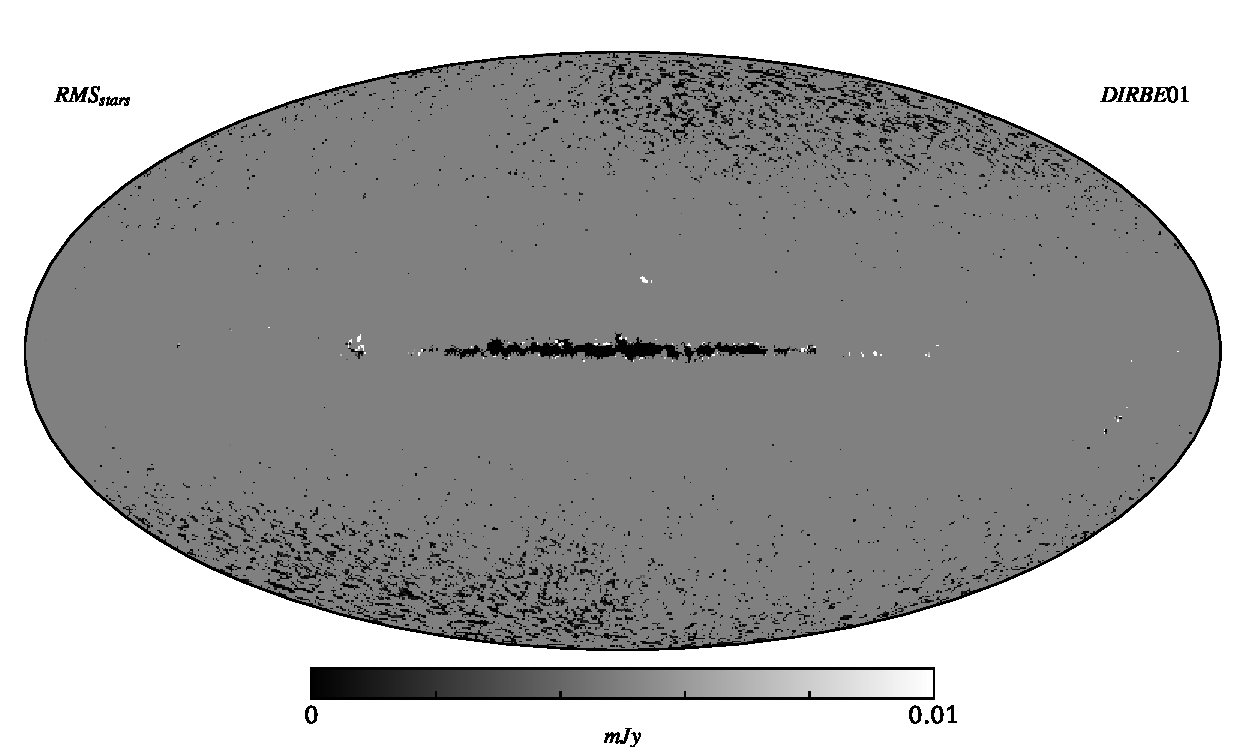
\includegraphics[width=0.49\columnwidth]{figs/stars_std_01.pdf}
%  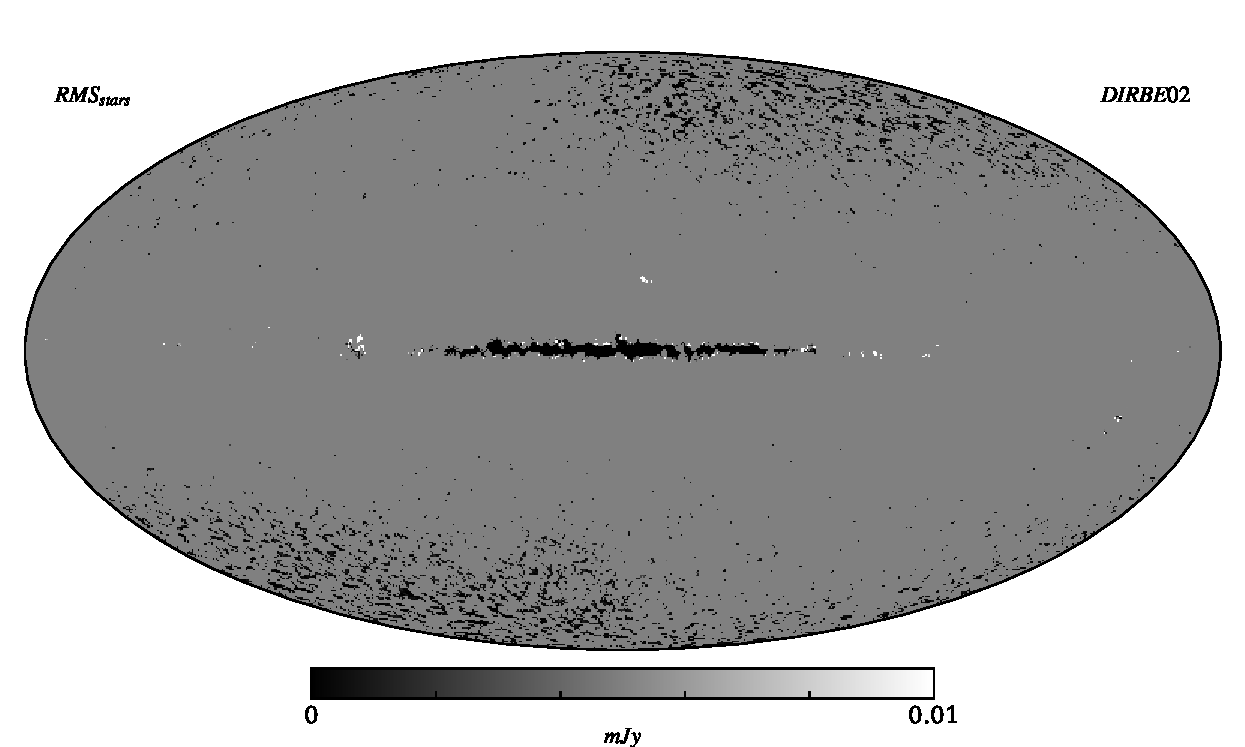
\includegraphics[width=0.49\columnwidth]{figs/stars_std_02.pdf} \\
%  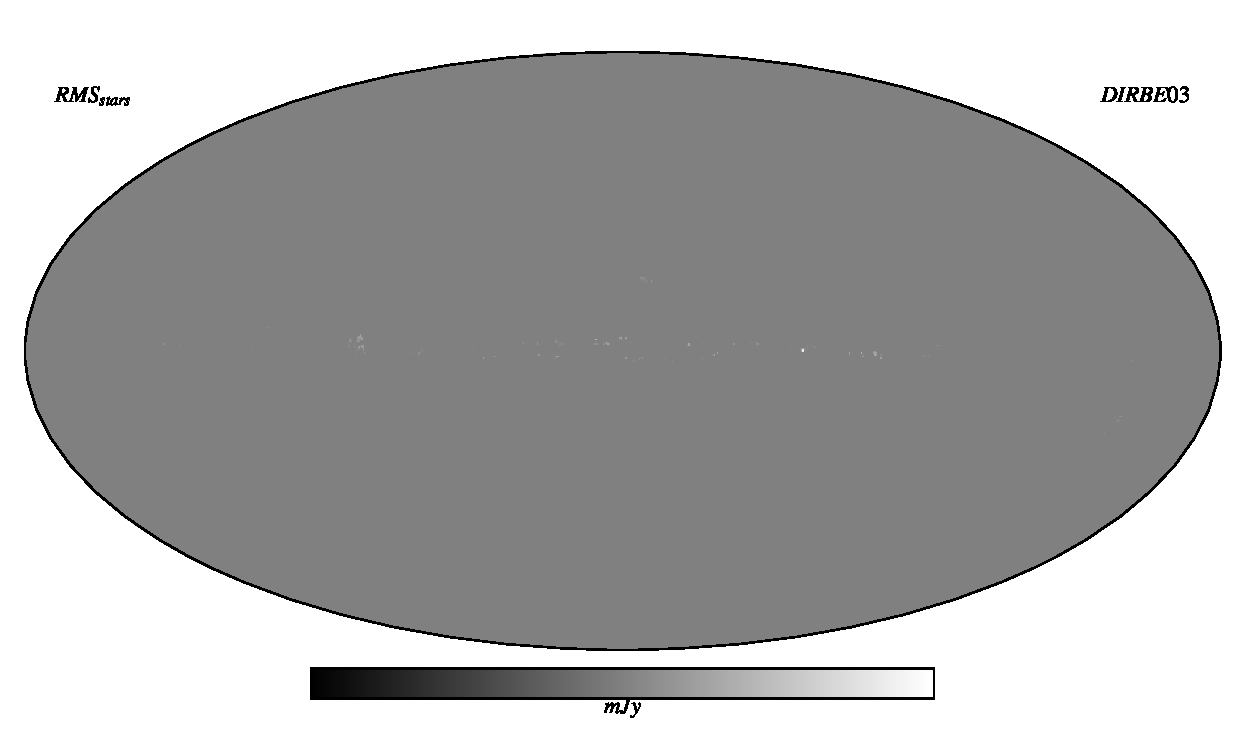
\includegraphics[width=0.49\columnwidth]{figs/stars_std_03.pdf}
%  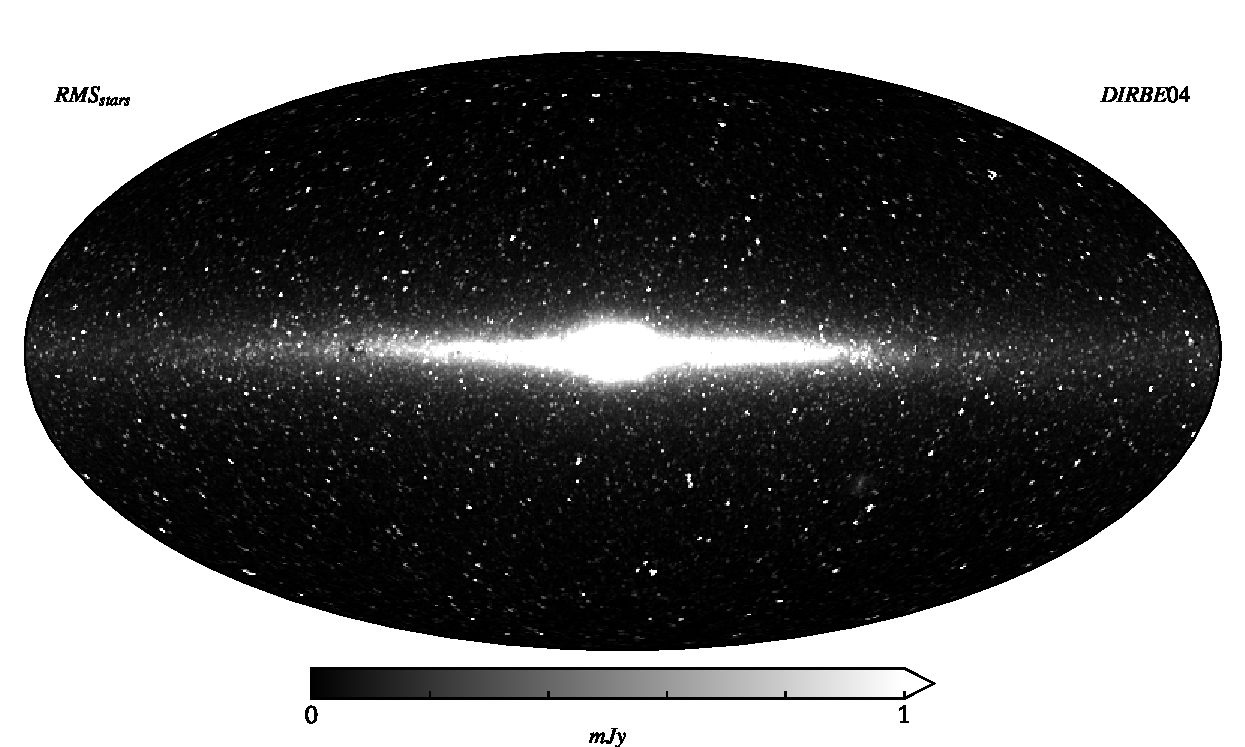
\includegraphics[width=0.49\columnwidth]{figs/stars_std_04.pdf} \\
%  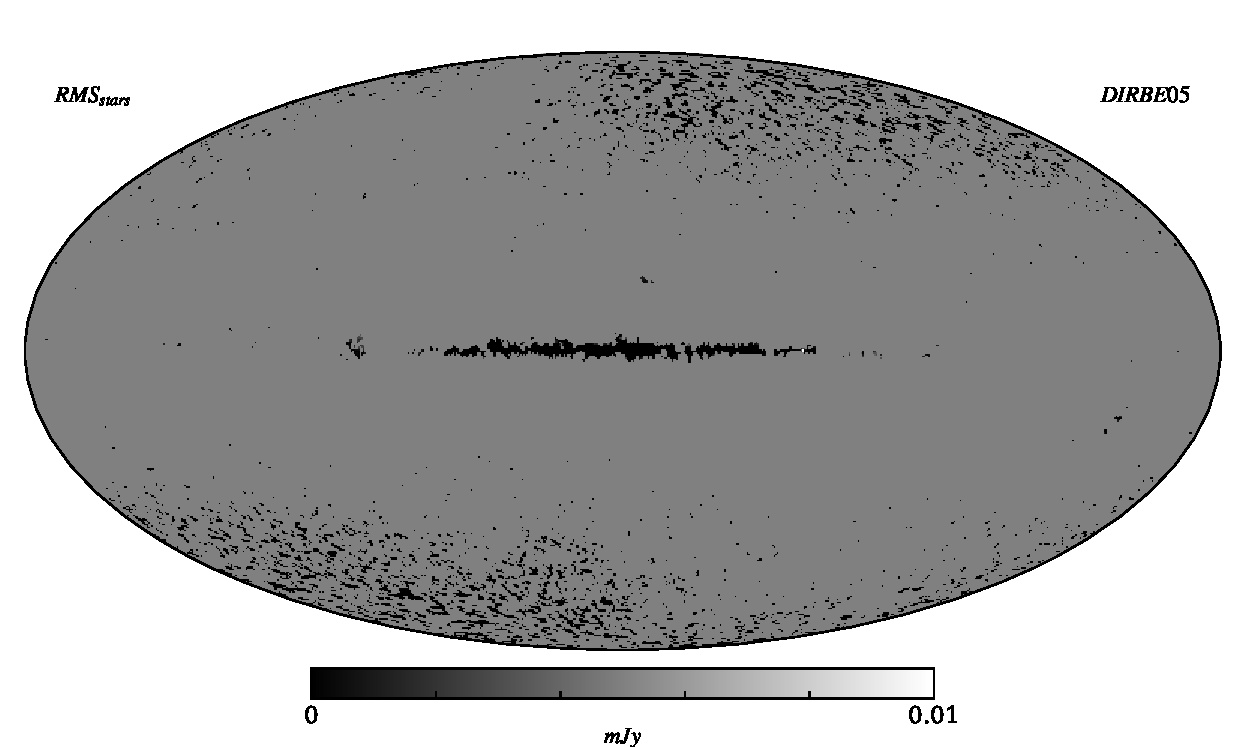
\includegraphics[width=0.49\columnwidth]{figs/stars_std_05.pdf}
%  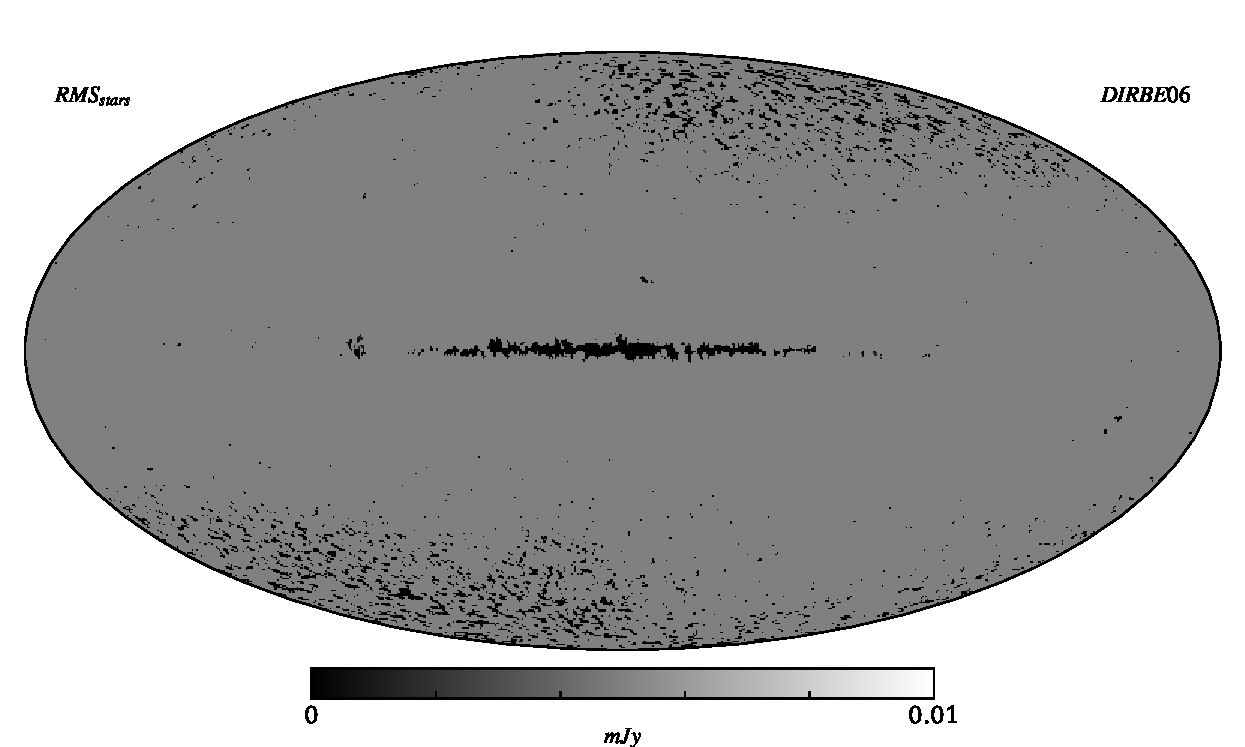
\includegraphics[width=0.49\columnwidth]{figs/stars_std_06.pdf} \\
  \caption{Standard deviation star maps from the Cosmoglobe DR2 release for the first 6 DIRBE bands. }
  \label{fig:std}
\end{figure*}


Figure: all star fits as a function of frequency 

\clearpage
\section{Conclusions}
\label{sec:conclusions}

Stars are a critical component of the infrared sky, which must be correctly modelled in order to avoid contaminating other components. 

\subsection{Future Work}

Including the WISE data directly in the full run would be an important next step, and could potentially give enough extra information to constrain the star SEDs directly instead of pre-computing them. 




\begin{acknowledgements}
 The current work has received funding from the European
  Union’s Horizon 2020 research and innovation programme under grant
  agreement numbers 819478 (ERC; \textsc{Cosmoglobe}) and 772253 (ERC;
  \textsc{bits2cosmology}). Some of the results in this paper have been derived using the HEALPix \citep{HEALPIX} package.
  We acknowledge the use of the Legacy Archive for Microwave Background Data
  Analysis (LAMBDA), part of the High Energy Astrophysics Science Archive Center
  (HEASARC). HEASARC/LAMBDA is a service of the Astrophysics Science Division at
  the NASA Goddard Space Flight Center.  
\end{acknowledgements}


%-------------------------------------------------------------
%                                       Table with references 
%-------------------------------------------------------------
%

\bibliographystyle{aa}
\bibliography{references, ../../common/CG_bibliography}
\end{document}
%%%% End of aa.dem
